\chapter{ヒストグラム}
\label{chap_Histogram}

\section{ヒストグラムとは何か}
ヒストグラム(histogram、度数分布図)は、ある物理量を複数回測定したとき、測定値の分布がどのようになっているかを表すときに頻繁に使われます。身近な例では、図\ref{fig_population_eps}に示すような人口の年齢分布などに使われます。

\begin{figure}
  \begin{center}
    \includegraphics[width=12cm,clip]{fig/population.eps}
    \caption{2005年国勢調査を元にした、全国合計、東京都、島根県の年齢別人口分布。コード\ref{code_frame_fill_color}で同じ結果を得られる。データは\url{http://www.e-stat.go.jp/SG1/estat/List.do?bid=000001007609&cycode=0}から入手可能。}
    \label{fig_population_eps}
  \end{center}
\end{figure}

ヒストグラムを使うと、その測定対象がどのような値を取りやすいのかが、一目瞭然になります。図\ref{fig_population_eps}の元データは、総務省統計局のまとめた国勢調査の結果です。コード\ref{code_population_dat}のような、単なる数字の羅列を見ただけでは、このデータがどのような特性を持っているのかを視覚的に認識することは大変困難です。どのような年齢層に人口が偏っているのか、東京のような都市部と鳥取のような地方では、人口分布の特徴がどうなっているのか、こういう情報はヒストグラムにして比較するのが一番です。図\ref{fig_population_eps}と図\ref{fig_population2_eps}は、コード\ref{code_population_C}で作成しました。

%\begin{NoFloat}
\lstinputlisting[language=TeX,float=tb,caption=\texttt{population.dat},label=code_population_dat,numbers=left]{src/population.dat}
%\end{NoFloat}

ヒストグラムを「読む」上で大切な点は、棒の1本ずつの面積が意味を持つということです。図\ref{fig_population_eps}を見ると、0〜5歳の人口は全国平均で約4.5\%になっています。ただし、縦軸の値は「\%」ではなく「\%/5 year」になっていることに注意してください。1つの棒の幅が5年間分あるので、縦軸の値に5年間をかけて、単位が「\%」になった人口の割合が出てくるわけです\footnote{新聞などで見かける図表の多くは、縦軸の単位を省略して単純に「\%」を使うことが多いですが、我々のように物理量を単位を含めて正確に扱う場面では、分母が何であるのか注意してください。}\footnote{図\ref{fig_population_eps}では、3つのヒストグラムを並べて表示するために棒の幅を5年間よりも細くしています。5年間分の太さにするほうがより正確な表現ですが、この図では(本来の幅が常識で判断できるため)見やすさを優先してあります。}。

\subsection{折れ線グラフとの違い}

ヒストグラムの用途は、ある測定値の範囲にどれだけの事象(イベント)が存在するかを図示することです。したがって、測定値には幅が存在し、特定の測定値で代表することはできません。先ほどの図\ref{fig_population_eps}の例では、最初の棒は$0$〜$5$歳の人口を表していました。縦軸の値は、中心値の$2.5$歳を代表するものではないことに注意してください。

従って、図\ref{fig_population_eps}を図\ref{fig_population2_eps}のように折れ線グラフにして表示するのは誤りです。折れ線グラフにする場合は、1つ1つの点の座標がともに(誤差の範囲内で)意味のある1つの数値でなくてはいけません。折れ線グラフを使用するのは、原則として線分の傾きに意味がある場合に限ります。

\begin{figure}
  \begin{center}
    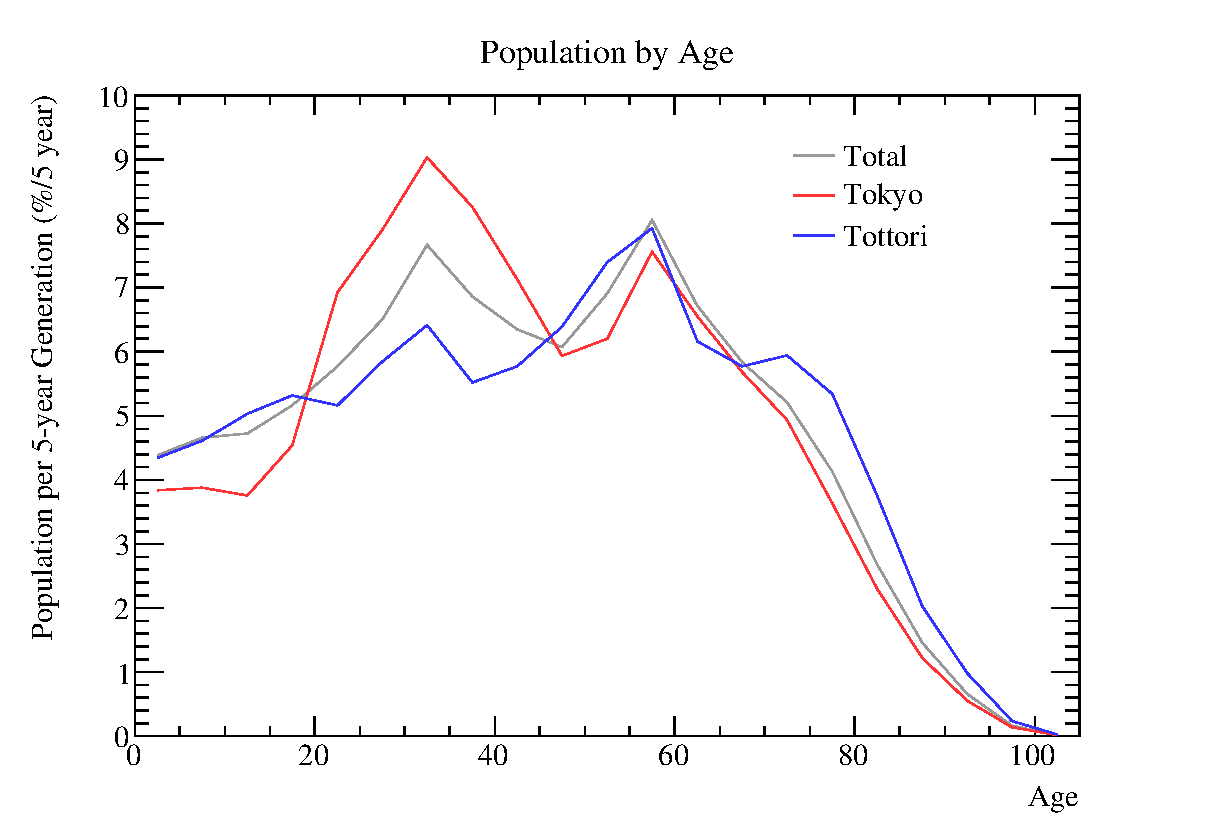
\includegraphics[width=12cm,clip]{fig/population2.eps}
    \caption{図\ref{fig_population_eps}の間違った表示方法の例}
    \label{fig_population2_eps}
  \end{center}
\end{figure}

\subsection{ビン}

図\ref{fig_population_eps}の横軸は、0〜105歳を21の区間に分けてあります。このような小分けした区間のことを、ビン(bin)と呼びます。またそれぞれのビンの幅が5歳分に相当し、これをビン幅(bin width)と呼びます。この例の21という数を、ビン数などと呼ぶことがあります。同じデータに対してビン数を変化させても、ヒストグラムの総面積は一定であることに注意してください。

\begin{NoFloat}
\lstinputlisting[language=c++,breaklines=true,caption=\texttt{population.C},label=code_population_C,numbers=left]{src/population.C}
\end{NoFloat}

\section{1次元ヒストグラム}


\section{2次元ヒストグラム}

\section{3次元ヒストグラム}
